\chapter{Information Extraction}\label{chapter:ie}
When \textbf{Filter} has confirmed the webpage is a target webpage, it will send a \texttt{new} command to \textbf{Extractor} through the socket communication. In this chapter, we will introduce another key part of the whole pipeline, information extraction, in detail.

As it shown in Figure \ref{fig:fc:extractor}, when the \textbf{Extractor} agent receive a HTML document, it first checks whether there exists records which have the same layout. If the number of the records is larger than a certain threshold, then we affirm that this item has already have a valid existing extractor instance. Thus, we can use this extractor instance to do feature extraction to this item directly. Otherwise, this record will be put into the extract list. With the help of our pre-trained extraction ontology, possible rules will be selected automatically from the rule library. Additionally, visualisation assists us fast amend these rules and create new rules and hence achieve the goal of extracting structured information.

Furthermore, if we find some items with wrong marked labels in the extract list, we can send \texttt{new} command to \textbf{Filter} again and with the addition of human decision.

\begin{figure}[htb!]
	\centering
	\includegraphics[page=7,width=0.9\textwidth]{images/diagrams.pdf}
	\caption{Flow Chart for Extractor}\label{fig:fc:extractor}
\end{figure}

As information extraction is the emphasis of this part, we divide the explanation into two steps in particular: attribute extraction and entity extraction. As a matter of fact, when we finish attribute extraction, entity extraction will combine those attributes together to form an entity.

\section{Attribute Extraction}
\begin{defn}
An Extraction Rule for a specific attribute $a$:
\begin{equation}
	r_a = \langle \mathcal{S}_G, \mathcal{S}_L,M, H, T, \mathcal{A} \rangle
\end{equation}
 where:
\begin{itemize}
	\item $\mathcal{S}_G$ is a global selector, it will pick a specific part of a HTTP response, it can be:
		\begin{itemize}
			\item content: the HTTP response body, i.e. the HTML content.
			\item url: the URL of the HTTP response. 
			\item title: the title of the HTML document. 
		\end{itemize}
	\item $\mathcal{S}_L$ is a scope selector, it will only exist when $\mathcal{S}_G=content$. This selector is implemented as CSS selectors, so it can indicate specific DOM node in the HTML DOM tree. It also need point out to keep the html or just text after this selection.
	\item $M$ is a regular expression, which is to match some parts from the target scope.
	\item $H$ and $T$ are regular expressions, which denoted the pre-indicator and post-indicator respectively, i.e. the content before and after the target result.
	\item $\mathcal{A}$ is a set of predefined actions, e.g. \code{strip} and \code{parseDate} which will be applied to the final extraction result. 
\end{itemize}
\end{defn}

In some cases, specific attribute may not included in the target page, so we especially define a \textit{undefined rule} as $r_0$. $r_0$ will also applied to the attribute where the rule hasn't been selected.

In order to make the rule understandable for the system, we give a ontology representation for extract rule in XML format. The \code{on} attribute in the \code{rule} node is the global selector $\mathcal{S}_G$,
\vspace{1em}
\lstinputlisting[language=xml,caption=Ontology Representation for Extraction Rule]{./src/onto_rule.xml}

For an HTTP Response, if we extract an attribute $a$ by following an attribute extract rule $r_a=\langle \mathcal{S}_G, \mathcal{S}_L, M, H, T, \mathcal{A} \rangle$, then as it is shown in Figure \ref{fig:attribute_ext}, $S_G$ will firstly extract the content part or URL part from the response. If $S_G = content$, then $S_L$ will utilise css selector to select a particular scope in order to further narrowing the scope of the target. After matching pattern from the scope by $M$, use two regular expressions, $H$ and $T$, to extract the target successively. At last, some pre-defined actions will be applied on these target string. And we list some of our pre-defined actions in Table \ref{tab:actions}
\begin{figure}[htb!]
	\centering
	\includegraphics[page=10,width=0.9\textwidth]{images/diagrams.pdf}
	\caption{Attribute Extract}\label{fig:attribute_ext}
\end{figure}

\begin{table}[htb!]
\small
\centering
\caption{Pre-defined Actions in Attributes Extraction}
\label{tab:actions}
\resizebox{\textwidth}{!}{%
\begin{tabular}{@{}p{0.1\textwidth}p{0.35\textwidth}p{0.4\textwidth}@{}}
\toprule
\textbf{ID} & \textbf{Name} & \textbf{Description} \\ \midrule
$a_1$ 
	& \texttt{removeHTML} 
	& remove all HTML tags in the target string
	\\ \midrule
$a_2$ 
	& \texttt{stripe}
	& remove the blank character(space/tab/newline) at the beginning and end of the target string
	\\ \midrule
$a_3$ 
	& \texttt{parseDate}
	& parse the target string into a specific fixed date format. It is convenient for us to save them into the database uniformly and helps with the query afterwards.
	\\ \midrule
$a_4$ 
	& \texttt{parseTime}
	& parse the target string into a specific fixed time format. It is convenient for us to save them into the database uniformly and helps with the query afterwards.
	\\ \bottomrule
\end{tabular}
}
\vspace{-1em}
\end{table}

Based on the definition of the attribute extraction rule, we can define a rule set for a particular attribute. Different rules in a rule set are aiming at the same feature in different webpages.
\begin{defn}
A Rule Set for a specific attribute $a$:
\begin{equation}
	\mathcal{R}_a = \lbrace \text{ $r$ $\vert$ $r$ is an Attribute Extraction Rule for attribute $a$}  \rbrace
\end{equation}
\end{defn}

We use the following presentation format in XML.
\lstinputlisting[language=xml,caption=Ontology Representation for Attribute Rule Set]{./src/onto_ruleset.xml}

\section{Entity Extraction}
\begin{defn}
An Extractor Instance $E$ is a permutation of list of attribute extract rule $r$, each $r$ corresponds to a specific attribute of the entity:
	\begin{equation}
		E = \mathcal{R}_{a_1} \times \mathcal{R}_{a_2} \times ... \times \mathcal{R}_{a_n}
	\end{equation}
\end{defn}

For the purpose of recording an extractor conveniently, we provide a serialisation of it. It uses a string which contains id of every attribute extraction rule to represent an extractor instance. For example, $E=1,3,1$ means for an entity, use $r_1 \in \mathcal{R}_1$ to extract the first attribute, $r_3 \in \mathcal{R}_2$ to extract the second attribute and $r_1 \in \mathcal{R}_3$ to extract the third attribute.

Particularly, we designed the ontology(XML Format) below for Seminar Announcement\footnote{The XML Schema for extract entity is given in the Appendix \ref{apdx:ie_onto}}. It connects with the attribute extraction rule set we introduced above, and contains name of each attribute \texttt{name}, field names of database \texttt{db-col}, \texttt{description}, and length limitation \texttt{max-len} etc. Meanwhile, \texttt{title.xml} and \texttt{location.xml} are both ontology files of attribute extraction rule set which for corresponding attributes.

\lstinputlisting[language=xml,caption=Ontology Representation for Seminar Entity]{./src/seminar_eneity.xml}

\section{Visual-aid Rule Generation}
Next, we are going to explain how to create and use these rules and extractor instances. During the entire extraction process, attribute extraction rule is the most basic component. But for users, attribute extraction rule is still very complex. Under the situation that it is hardly possible to reduce the complexity, we introduce visualisation as an assistance. This method not only helps user create correct attribute extraction rule easily and efficiently, but also be convenient for amending rules visually. In addition, information extraction rule involves some basic knowledge in html and regular expression. As these are rather simple and easy to understand, we assume that our user was trained related knowledge(including basic HTML and regular expressions).
\begin{figure}[htb!]
	\centering
	\includegraphics[page=8,width=\textwidth]{images/picture.pdf}
	\caption{Extractor List and Modal View}\label{fig:ext:list_and_modal}
\end{figure}

When we open an item waiting to be extracted in the extractor list, a modal view (see Figure \ref{fig:ext:list_and_modal}) will show up. This modal preview window is the main graphical user interface where the user conducts information extraction. It is consist of three main parts:
\begin{enumerate}
  \item The left division is a preview of the webpage, it can be used to look up the original webpage as well as its source code. 
  \item The upper part of the right division is the rule selection area. It is responsible for the function of creating and selecting rules. The lower half is a fast tabular preview. Both these two parts of the right division are generated automatically according the the extraction ontology, which means they could be easily migrate to other scenarios.
\end{enumerate}

End users can choose rules for different attributes in the rule selection area quickly according to different attributes of the various rule set. When clicking on a single rule, Web Interface will send \texttt{preview} to the \textbf{Extractor}. After receiving the response, the tabular preview at bottom will update the content to present what has been extracted by this rule. however, by using this method alone, normal users are hard to find where the problem sits if any rule is not applicable or simply goes wrong. Thus, we use visualisation to show the extracted area of a rule in the left webpage preview part.

We designed a set of glyph to represent different attributes in order to make the visualisation of webpage preview be more intuitive and contain more information(in Figure \ref{tab:glyph}). Applying glyph could help the text and the data variables be processed using pre-attentive visual search\cite{tory2004human}. By injecting javascript code into the original webpage, we carried out inserting visualisation element(including both glyph and other elements) into the preview webpage dynamically. This helps the user get feedbacks more visually.

\begin{table}[htbp!]
\small
\centering
\caption{Glyph Visualisation Elements}
\label{tab:glyph}
\resizebox{\textwidth}{!}{%
\begin{tabular}{@{}p{0.1\textwidth}p{0.2\textwidth}|p{0.1\textwidth}p{0.2\textwidth}|p{0.1\textwidth}p{0.2\textwidth}@{}}
\toprule
\textbf{Glyph} & \textbf{Attribute} & \textbf{Glyph} & \textbf{Attribute} & \textbf{Glyph} & \textbf{Attribute} \\ \midrule
\includegraphics[width=36px]{images/icon/title} 
	& \texttt{title}& 
\includegraphics[width=36px]{images/icon/speaker} 
	& \texttt{speaker}& 
\includegraphics[width=36px]{images/icon/location} 
	& \texttt{location}
	\\ \midrule

\includegraphics[width=36px]{images/icon/date} 
	& \texttt{date}& 
\includegraphics[width=36px]{images/icon/time} 
	& \texttt{time}& 
\includegraphics[width=36px]{images/icon/abstract} 
	& \texttt{abstract}
	\\ \bottomrule
\end{tabular}
}
\end{table}

Furthermore, creating a new attribute extract rule is also very easy under this kind of mechanism. User only needs to choose tabs in the rule selection area to add new rules to the rule set (corresponding to an attribute), and click `create a new rule' afterwards. Then, user is able to create new rules for an extracting attribute fast and accurately based on the form below and the visualisation feedback.\\

\noindent\begin{minipage}{0.5\textwidth}
\includegraphics[page=9,width=\textwidth]{images/picture.pdf}
\end{minipage}
\hfill
\begin{minipage}{0.5\textwidth}
\begin{enumerate}
	\item At first, we can choose a particular part(\textit{content}, \textit{title} or \textit{url}) where the new rule will be applied in the ``On" field. This is the $S_G$ we defined before. Normally, except that attributes such as \texttt{title} will be contained in the webpage's title, most attributes are in the html content.
	\item If extracting from html content, we can create a css selector in the ``Scope" field based on the webpage's html structure and source code so that we could select the scope (a DOM tree node) which contains the target content in html. This is the $S_L$ which we defined before. Additionally, we are able to decide to keep html or text for the chosen scope.
\end{enumerate}
\end{minipage}

\begin{enumerate}
\setcounter{enumi}{2}
	\item The field Match($M$) can get a matching result from the target scope by using regular expression. This is especially suitable for attributes with fixed format, such as \texttt{date} and \texttt{time}.
	\item On the other hand, we can do before and after interception to the target content. In order to proceed this, we need to set the regular expressions for head($H$) and tail($T$) in the ``After" and ``Before" fields correspondingly.
	\item After that, we can tick some items in the ``Post Action" Field to set the $\mathcal{A}$ we defined before and conduct post-process to the target we extracted.
	\item Finally, for the purpose of recognising this rule, we add a short introduction in the field ``Description" to describe this rule for later usage.
\end{enumerate}

After completing the rule creation form, Web Interface will send \texttt{test\_rule} to the \textbf{Extractor} by clicking the `test' button. The system will provide feedback in both test result area and webpage preview area (see Figure \ref{fig:ext:aer_vf}). In the webpage preview area, firstly, the injected javascript will add a highlight border to parts of the text which were selected by the combination of $S_G$ and $S_L$. Then the glyph we designed will be added to the beginning and end of the target string. In fact, this is because the javascript we injected has modified the html code of the original webpage(shown as in Figure \ref{fig:ext:ve_inject}). Just like Figure \ref{fig:ext:aer_vf}, first add a border to the \texttt{.date-display-single} scope; then add \texttt{img} which contains glyph to both left end and right end of the extracting target ``Wednesday, 28 October".

\begin{figure}[htb!]
	\centering
	\includegraphics[page=10,width=\textwidth]{images/picture.pdf}
	\caption{Attribute Extract Rule and Visualisation Feedback}\label{fig:ext:aer_vf}
\end{figure}

\begin{figure}[htb!]
	\centering
	\includegraphics[page=11,width=0.7\textwidth]{images/picture.pdf}
	\caption{Visualisation Element Inject}\label{fig:ext:ve_inject}
\end{figure}

If the selected area does not exist, the system will warn the user directly. This mechanism helps user understand the problem of the rule more conveniently so that user can correct it in time. If user is satisfied with this new rule, then he can click on the `add' button to send \texttt{add\_rule} to \textbf{Extractor} so that this new rule will be added to the corresponding attribute rule set.

That is how to select or create an attribute extraction rule. When the extraction rule for each attribute has been set up, user can choose or create an appropriate extractor instance for a particular webpage on account of different attributes. We can see the extracting result through the preview table in real-time. If the result is satisfactory, user will click the `extract' button to send \texttt{add\_extractor} to \textbf{Extractor}. Once the \textbf{Extractor} receives this message, it will automatically serialise the id of these attribute extraction rules to form an extractor instance. This extractor instance will be bound with this url and stored into \texttt{url\_lib}. Meanwhile, the target information in this webpage will be extracted based on this extractor and saved into \texttt{sem\_info}.

\section{Show Cases}
Here, we carefully chose three representative examples which are suitable for demostration. We will give the extract rule, visualisation and the extracted result of each example correspondingly.

Before we start, in order to show the attribute extract rule clearly, we define the string format of attribute extract rule $r_{attr} = \langle \mathcal{S}_G, \mathcal{S}_L,M, H, T, \mathcal{A} \rangle$ for attribute $attr$ is:
\begin{figure}[htb!]
	\centering
	\includegraphics[page=26,width=0.5\textwidth]{images/picture.pdf}
\end{figure}

\noindent \textbf{Example 1:}\\
url: http://www.cs.ox.ac.uk/seminars/1429.html\\
title: Department of Computer Science, University of Oxford: Tree Buffers
\begin{figure}[htbp!]
	\centering
	\includegraphics[page=21,width=0.85\textwidth]{images/picture.pdf}
	\caption{Information Extraction Show Cases 1: Webpage}\label{fig:ie_case_1b}
\end{figure}

We could easily find in Figure \ref{fig:ie_case_1b} that \texttt{title} can be extracted from the webpage's title. And \texttt{date}, \texttt{time}, \texttt{location} and \texttt{abstract} are all following to the corresponding indicator words. In other words, except of \texttt{speaker}, all other data could be extracted by using indicators directly. Hence, our rule should take full advantage	of the pre and post interception of $H$ and $T$. Below is our extracting rule and result.

\begin{figure}[htbp!]
	\centering
	\includegraphics[page=20,width=\textwidth]{images/picture.pdf}
\end{figure}

We visualised these rules in Figure \ref{fig:ie_case_1v}.
\begin{figure}[H]
	\centering
	\includegraphics[page=22,width=0.60\textwidth]{images/picture.pdf}
	\caption{Information Extraction Show Cases 3: Visualisation}\label{fig:ie_case_1v}
\end{figure}


\noindent \textbf{Example 2:}\\
url: http://www.pharm.ox.ac.uk/seminars/michaelmas-seminars/2013/of-genes-and-brains-neurotrophism-in-drosophila\\
title: Of genes and brains: neurotrophism in Drosophila — Pharmacology\\

\begin{figure}[htbp!]
	\centering
	\includegraphics[page=24,width=\textwidth]{images/picture.pdf}
	\caption{Information Extraction Show Cases 2: Webpage and Source Code}\label{fig:ie_case_2b}
\end{figure}

In this example, it can be seen from Figure \ref{fig:ie_case_2b} that the DOM Nodes contains core attributes in this webpage's source code can be distinguished through tag id or class. Thus, this rule are mainly relied on css selector, i.e. $S_L$. There are two things we need to give a special explanation:
\begin{itemize}
	\item For the attribute \texttt{date}, the target we get is the value of \texttt{title} of the DOM Node whose class is \texttt{dtstart}.
	\item As the webpage did not provide \texttt{abstract}, the rule for \texttt{abstract} is \textit{undefined rule}($r_0$). Therefore, the extracted result of it in the entity is also empty.
\end{itemize}

We got the following rules and results:
\begin{figure}[htbp!]
	\centering
	\includegraphics[page=23,width=\textwidth]{images/picture.pdf}
\end{figure}

We visualised these rules in Figure \ref{fig:ie_case_2v}
\begin{figure}[H]
	\centering
	\includegraphics[page=25,width=\textwidth]{images/picture.pdf}
	\caption{Information Extraction Show Cases 2: Visualisation}\label{fig:ie_case_2v}
\end{figure}

\pagebreak
\noindent \textbf{Example 3:}\\
url: http://www.dpag.ox.ac.uk/seminars/metabolism-hypoxia-and-the-diabetic-heart\\
title: Metabolism, hypoxia and the diabetic heart — Physiology, Anatomy and Genetics\\

\begin{figure}[htbp!]
	\centering
	\includegraphics[page=18,width=0.85\textwidth]{images/picture.pdf}
	\caption{Information Extraction Show Cases 3: Webpage and Source Code}\label{fig:ie_case_3b}
\end{figure}

From Figure \ref{fig:ie_case_3b}, we could find that the attributes of this webpage do not follows the indicators. So the extract rules for this webpage will be more depend on the structure and content of html. We created the following rules based on the webpage's source code and got the ideal extraction results.

\begin{figure}[htbp!]
	\centering
	\includegraphics[page=17,width=\textwidth]{images/picture.pdf}
\end{figure}

We visualised these rules in Figure \ref{fig:ie_case_3v}
\begin{figure}[htbp!]
	\centering
	\includegraphics[page=19,width=0.85\textwidth]{images/picture.pdf}
	\caption{Information Extraction Show Cases 3: Visualisation}\label{fig:ie_case_3v}
\end{figure}

\pagebreak
\section{Automatic Pick Extractor}
As we stated above, when the system has extracted a certain number of webpages, \textbf{Extractor} will be able to select extractor instance for new webpages automatically, which greatly reduces the user operation. Specifically, it is implemented by comparing the layouts.

\begin{defn}\label{defn:layout}
In our system, the Layout of a webpage means the skeleton of HTML . The system will delete the content-related parts in html. Specifically, it contains the following possibilities:
	
\begin{table}[htb!]
\small
\centering
\caption{Content-related Elements in HTML}
\label{tab:layout_content}
\begin{tabular}{@{}p{0.3\textwidth}p{0.7\textwidth}@{}}
\toprule
\textbf{Elements} & \textbf{Example \& Explanation} \\ \midrule
Text in DOM leaf node 
	& \code{<p>content<p>} $\rightarrowtail$ \code{<p><p>}
	\\ \midrule
\texttt{head} tag in HTML 
	& \code{<html><head>...</head><body>...</body></html>} $\rightarrowtail$ \code{<html><body>...</body></html>}
	\\ \midrule
Comments in HTML 
	& \code{<!--something-->} $\rightarrowtail$ $\dag$
	\\ \midrule
Specific tags in HTML 
	& \code{"script", "map", "p", "link", "meta", "img", "br", "head", "span", "a", "h1", "h2", "h3", "h4",
                     "h5", "h6", "li", "input"} $\rightarrowtail$ $\dag$
	\\ \midrule
Specific attributes in HTML 
	& \code{"name", "content", "src", "href", "id", "type", "action", "rel", "placeholder", "style", "for", "data.*?", "onclick", "onmouseover", "alt", "title", "value", "onblur", "autocomplete", "maxlength", "onfocus", "usemap", "media", "itemscope"} $\rightarrowtail$ $\dag$
	\\ \bottomrule
\end{tabular}
\end{table}
By deleting content-related part in the HTML file, we thereby get the Layout of that webpage.
\end{defn}


In order to compare the layouts more efficiently, we hash the layout and store the hash value into \texttt{url\_lib} as an attribute of HTTP response. If the number of the same layout and mutual extractor instance in the database goes beyond the threshold, this extractor will be automatically allocated to this item to do extraction. We call this extractor `valid existing extractor'.

\section{Extractor List Refresh}
After the system completes extractor instance selection on some items with the manual assistance, some items in the extractor list may have reached the requirement of automatic pick extractor, i.e. the valid existing extractor has already existed. Therefore, user can click the refresh extractor button at left to send \texttt{refresh} command to \textbf{Extractor}. Once \textbf{Extractor} receives this command, it will rejudge each item in the extract list. If a valid existing extractor is discovered, \textbf{Extractor} will directly bind this extractor and start extracting.

\begin{figure}[htb!]
	\centering
	\includegraphics[page=16,width=0.3\textwidth]{images/picture.pdf}
\end{figure}

\section{Visualisation for Extraction Result}
All the results we got through the solution above will be store in the table `sem\_info'. Then, although this is not the key point of our project, we still implemented a Presenter to present these information. As stated before, we use a present way that in line with the characteristics of seminar announcements, which is calendar. The events in this calendar are the seminar announcements we extracted. And these events will be automatically updated when the database updates. Users can easily get access to view all the recent seminars, compare availability and manage attendance.
\begin{figure}[htbp!]
	\centering
	\includegraphics[page=13,width=\textwidth]{images/picture.pdf}
	\caption{Result Visualisation: Three Views}\label{fig:calender_views}
\end{figure}

In order to give a presentation with changeable data granularity, we provide three views: week, day and month. Here, considering the space limitation, we give some presentations on partial pages(see Figure \ref{fig:calender_views}).

The figure above shows a time based layout. In addition, we could open a modal view to check detail time of seminars by clicking the blocks in the views above. See Figure \ref{fig:calendar_inst} as an example. User will be able to see the information about title, start time, location, speaker and abstract etc. of a specific seminar. The URL of this announcement webpage will also be given at bottom.

\begin{figure}[htb!]
	\centering
	\includegraphics[page=14,width=0.65\textwidth]{images/picture.pdf}
	\caption{Result Visualisation: Calendar}\label{fig:calendar_inst}
\end{figure}










